\section{Experimental results}
\label{sec:experimental_results}
The proposed architecture is demonstrated on a Xilinx Zynq-7020. This device integrates a dual ARM Cortex-A9 based processing system (PS) and programmable logic (PL) equivalent to Xilinx Artix-7 (FPGA) in a single chip \cite{xilinx2015zynq}. The Zynq-7020 architecture conveniently maps the custom logic and software in the PL and PS respectively as an embedded system.

In this platform, we implement the proposed hardware architecture to deploy the SbS network structure shown in \fig{fig:sbs_network} for handwritten digit classification task using MNIST data set. The SbS model is trained in Matlab without any quantization method, using standard floating-point. The resulting synaptic weight matrices are deployed on the embedded system. There, the SbS network is built as a sequential model using the API from the SbS embedded software framework \cite{nevarez2020accelerator}. This API allows to configure the computational workload of the neural network, which can be distributed among the hardware processing units and the CPU.

For the evaluation of our approach, we address a design exploration by reviewing the computational latency, inference accuracy, resource utilization, and power dissipation. First, we benchmark the performance of SbS network simulation on the embedded CPU, and then repeat the measurements on hardware processing units using standard floating-point computation. Afterwards, we evaluate our dot-product architecture, addressing a design exploration using custom floating-point, as well as the logarithmic computation. Finally, we present a discussion of the presented results.

\begin{figure}[!h]
	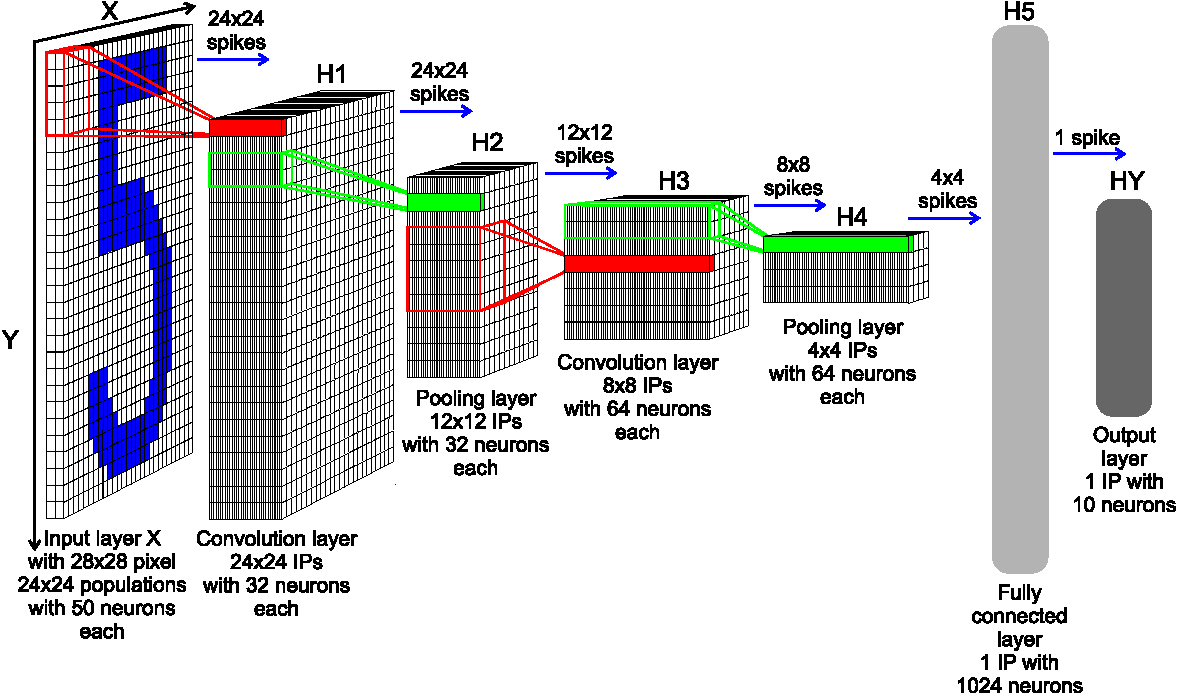
\includegraphics[width=\columnwidth]{../figures/sbs_network.pdf}
	\caption{SbS network structure for MNIST classification task.
		Input \emph{X}: Input layer with $28\times28$ normalization modules for $28\times28$ input pixel. From this layer spikes are send to layer \emph{H1}. \emph{H1}: Convolution layer \emph{H1} with $24\times24$ IPs with $32$ neurons each. Every IP processes the spikes from $5\times5$ spatial patches of the input pattern ($x$ and $y$ stride is $1$). \emph{H2}: $2\times2$ pooling layer \emph{H2} ($x$ and $y$ stride is $2$) with $12\times12$ IPs with $32$ neurons each. The weights between \emph{H1} and \emph{H2} are not learned but set to a fixed weight matrix that creates a competition between the \emph{32} features of \emph{H1}. \emph{H3}: $5\times5$ convolution layer \emph{H3} ($x$ and $y$ stride is $1$) with $8\times8$ IPs. Similar to \emph{H1} but with $64$ neuron  	for each IP. \emph{H4}: $2\times2$ pooling layer \emph{H4} ($x$ and $y$ stride is $2$) with $4\times4$ IPs with $64$ neurons each. This layer is similar to layer \emph{H2}. \emph{H5}: Fully connected layer \emph{H5}. $1,024$ neurons in one big IP which are fully connected to layer \emph{H4} and output layer \emph{HY}. \emph{HY}: Output layer \emph{HY} with $10$ neurons for the $10$ types of digits. selected.}\label{fig:sbs_network}
\end{figure}



\subsection{Performance benchmark}
\subsubsection{Benchmark on CPU}

We examine the performance of the CPU for SbS network simulation with no hardware coprocessing. In this case, the embedded software builds the SbS network as a sequential model mapping the entire computation to the CPU (ARM Cortex-A9) at 666 MHz and a power dissipation of $520 mW$.

The SbS network computation on the CPU achieves a latency of $34.3 ms$ per spike with an accuracy of 99.3\% correct classification on the $10,000$ image test set at $1000$ spikes. The latency and schedule of the SbS network computation are displayed in \Tab{tab:latency_sw} and \fig{fig:latency_sw} respectively.

\begin{table}[!t]\centering
	\caption{Computation on CPU.}\label{tab:latency_sw}
	\scriptsize
\begin{tabular}{lrr}\toprule
	\textbf{Layer} &\textbf{Latency (ms)} \\\midrule
	HX\_IN &1.184 \\
	H1\_CONV &4.865 \\
	H2\_POOL &3.656 \\
	H3\_CONV &20.643 \\
	H4\_POOL &0.828 \\
	H5\_FC &3.099 \\
	HY\_OUT &0.004 \\
		
	TOTAL &34.279 \\
	\bottomrule
\end{tabular}
\end{table}

\begin{figure}[t!]
	\centering
	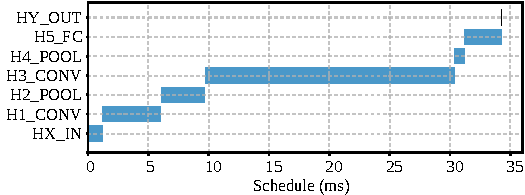
\includegraphics[width=1\columnwidth]{../figures/latency_sw.pdf}
	\caption{Computation on CPU.}
	\label{fig:latency_sw}
\end{figure}

\subsubsection{Benchmark on processing units using standard floating-point}
To benchmark the computation on hardware PUs using standard floating-point, we implement the system architecture shown in \fig{fig:hw_sbs_8_pu}. In this case, the embedded software builds the SbS network as a sequential model mapping the network computation to the hardware processing units at 200 MHz as clock frequency.

\begin{figure}[h!]
	\centering
	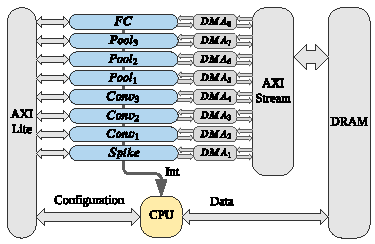
\includegraphics[width=0.5\textwidth]{../figures/sbs_hw_experimental.pdf}
	\caption{System overview of the top-level architecture with 8 processing units.}
	\label{fig:hw_sbs_8_pu}
\end{figure}

The layers of the neural network with the most neurons are partitioned for asynchronous parallel processing. Since \emph{H2\_POOL} and \emph{H3\_CONV} are the layers with the most neurons, the computational workload is distributed between two PUs for each one of these layers. The output layer \emph{HY\_OUT} is fully processed by the CPU, since it is the layer with fewer neurons. The hardware mapping and the computation schedule of this deployment are displayed in \Tab{tab:latency_fp} and \fig{fig:latency_pu_fp}.

\begin{table}[!t]\centering
	\caption{Performance of processing units using standard floating-point computation.}\label{tab:latency_fp}
	\scriptsize
	\begin{tabular}{llrrrrrr}\toprule
		\multicolumn{2}{c}{\textbf{Hardware mapping}} & &\multicolumn{4}{c}{\textbf{Computation schedule (ms)}} \\\cmidrule{1-2}\cmidrule{4-7}
		\textbf{Layer} &\textbf{PU} & &$t_s$ &$t_{CPU}$ &$t_{PU}$ &$t_f$ \\\midrule
		HX\_IN &Spike & &0 &0.056 &0.370 &0.426 \\
		H1\_CONV &Conv1 & &0.058 &0.598 &2.002 &2.658 \\
		\multirow{2}{*}{H2\_POOL}
		&Pool1 & &0.658 &0.126 &1.091 &1.875 \\
		&Pool2 & &0.785 &0.125 &1.075 &1.985 \\
		\multirow{2}{*}{H3\_CONV} 
		&Conv2 & &0.911 &0.280 &3.183 &4.374 \\
		&Conv3 & &1.193 &0.279 &3.176 &4.648 \\
		H4\_POOL &Pool3 & &1.473 &0.037 &0.481 &1.991 \\
		H5\_FC &FC & &1.512 &0.101 &1.118 &2.731 \\
		HY\_OUT &CPU & &1.615 &0.004 &0 &1.619 \\
		\bottomrule
	\end{tabular}
\end{table}

\begin{figure}[!t]
	\centering
	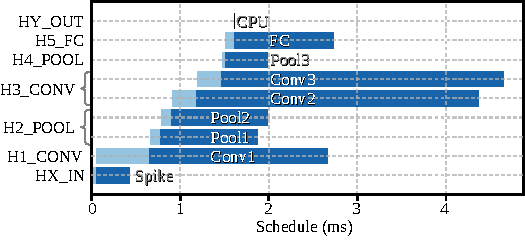
\includegraphics[width=1\columnwidth]{../figures/latency_pu_fp.pdf}
	\caption{Performance of processing units using standard floating-point computation.}
	\label{fig:latency_pu_fp}
\end{figure}

In the computation schedule, the following terms are defined as follows: $t_s(n)$ as the start time for the processing of the neural network layer (as a computation node) $n\in L$ where $L$ represents the set of layers; $t_{CPU}(n)$ as the CPU preprocessing time; $t_{PU}(n)$ as the PU latency; and $t_f(n)$ as the finish time. For data preparation, the $t_{CPU}(n)$ is the duration in which the CPU writes a DRAM buffer with $\vec{h_\mu}$ (vector of neuron latent variables) of the current processing layer and $\vec{S_t}$ (spike vector) from its preceding layer. This buffer is streamed to the PU via DMA.

The total execution time of the CPU is defined by \equ{eq:time_cpu}. In a cyclic spiking inference, the execution time of the network computation is the longest path among the processing units including the CPU. This is denoted as the latency of an spike cycle and it is defined by \equ{eq:time_spike}. The total execution time of the network computation is the last finish time defined by \equ{eq:time_finish}.

\begin{figure}[h!]
	\centering
	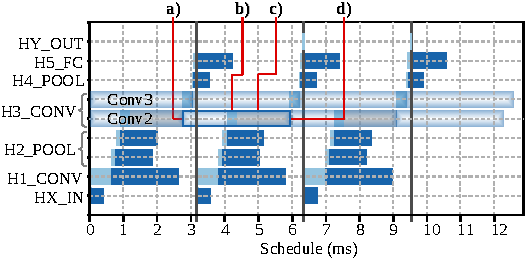
\includegraphics[width=1\columnwidth]{../figures/latency_fp_cycle.pdf}
	\caption{Performance bottleneck of cyclic computation on processing units using standard floating-point. a) Illustrates the starting of $t_{PU}$ of \emph{Conv2} on a previous computation cycle. b) Illustrates $t_{CPU}$ of \emph{Conv2} on the current computation cycle. c) Illustrates the CPU waiting time (in gray color) for \emph{Conv2} as a busy resource (awaiting for \emph{Conv2} interruption). d) Illustrates the $t_{f}$ from the previous computation cycle, the starting of $t_{PU}$ on the current computation cycle (\emph{Conv2} interruption on completion, and start current computation cycle).}
	\label{fig:latency_pu_fp_cycle}
\end{figure}

\begin{eqnarray} \label{eq:time_cpu}
T_{CPU} = \sum_{n\in L} t_{CPU}(n)
\end{eqnarray}

\begin{eqnarray} \label{eq:time_pu}
T_{PU} = \max_{n\in L}(t_{PU}(n))
\end{eqnarray}

\begin{eqnarray} \label{eq:time_spike}
T_{SC} =
\begin{cases}
T_{PU}, & \text{if}\ T_{CPU}\le T_{PU} \\
T_{CPU}, & \text{otherwise}
\end{cases}
\end{eqnarray}

\begin{eqnarray} \label{eq:time_finish}
T_{f} = \max_{n\in L}(t_{f}(n))
\end{eqnarray}

Using standard floating-point requires a high computational cost. As the largest layer, the computational workload of \emph{H3\_CONV} is evenly partitioned among two PUs: \emph{Conv2} and \emph{Conv3}. However, in the cyclic schedule, \emph{Conv2} causes the performance bottleneck as shown in \fig{fig:latency_pu_fp_cycle}. In this case, the CPU has to await for \emph{Conv2} to finish the computation of the previous cycle in order to start the current computation cycle. Applying \equ{eq:time_spike}, we obtain a latency of 3.183 ms per spike cycle. This deployment achieves an accuracy of $98.98\%$ correct classification on the $10,000$ image test set at $1000$ spikes.

The post-implementation resource utilization and power dissipation are shown in \Tab{tab:resource_fp} and \Tab{tab:power_fp}, respectively. Each \emph{Conv} PU instantiates an on-chip stationary weight matrix of $52,000$ entries to store $W\in\mathbb{R}^{5\times 5\times 2\times 32}$ and $W\in\mathbb{R}^{5\times 5\times 32\times 64}$ for \emph{H1\_CONV} and \emph{H3\_CONV}, respectively. In order to reduce BRAM utilization, we use a custom floating-point representation composed of 4-exponent and 4-bit mantissa. Each 8-bit entry is promoted to its standard floating-point representation for the dot-product computation. The methodology to find the appropriate bit width parameters for custom floating-point representation is presented in the next section.

\begin{table}[!h]\centering
	\caption{Resource utilization of processing units using standard floating-point.}\label{tab:resource_fp}
	\scriptsize
	\begin{tabular}{lrrrrrr}\toprule
		\textbf{PU} & &\textbf{LUT} &\textbf{FF} &\textbf{DSP} &\textbf{BRAM 18K} \\\midrule
		Spike & &2,640 &4,903 &2 &2 \\
		Conv & &2,765 &4,366 &19 &37 \\
		Pool & &2,273 &3,762 &5 &3 \\
		FC & &2,649 &4,189 &8 &9 \\
		\bottomrule
	\end{tabular}
\end{table}

\begin{table}[!h]\centering
	\caption{Power dissipation of processing units using standard floating-point.}\label{tab:power_fp}
	\scriptsize
	\begin{tabular}{lrr}\toprule
		\textbf{PU} &\textbf{Power (mW)} \\\midrule
		Spike &38 \\
		Conv &89 \\
		Pool &59 \\
		FC &66 \\
		CPU &520 \\
		\bottomrule
	\end{tabular}
\end{table}

\subsubsection{Benchmark on noise tolerance plot}
The noise tolerance plot serves as an intuitive visual model used to provide insights into accuracy degradation under approximate processing effects. This plot revels inherent error resilience, and hence, potential for approximation allowance. This plot offers an effective method to estimate the overall degradation of quality under applied approximation approaches, since both approximations and noise have qualitatively the same effect\cite{venkataramani2015approximate}.

In order to experimentally obtain the noise tolerance plot, we measure the inference accuracy of the neural network at increasing number of spikes. Then we repeat the measurements with uniformly distributed noise applied on the input images. We gradually ascend the levels of the noise amplitude, until accuracy degradation is detected. \fig{fig:accuracy_vs_noise_pu_fp} demonstrates this method using 100 sample images.

As benchmark, the tolerance plot in \fig{fig:accuracy_vs_noise_pu_fp} revels accuracy degradation after $50\%$ of noise amplitude and convergence with $400$ spikes. In this case, the particular SbS network with precise processing demonstrates a remarkable inherent error resilience, hence, a great opportunity for approximation.


\begin{figure}[h!]
	\centering
	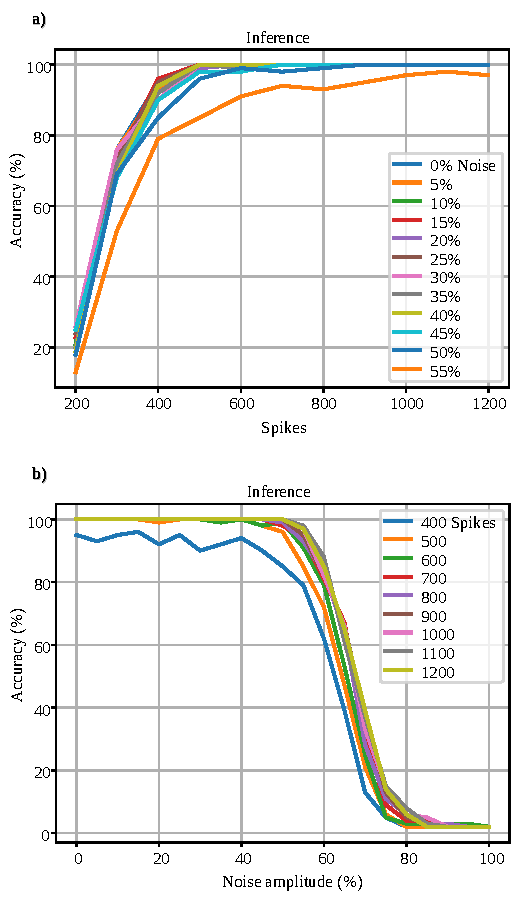
\includegraphics[width=1\columnwidth]{../figures/accuracy_vs_noise_pu_fp.pdf}
	\caption{Noise tolerance on hardware PU using standard floating-point computation (benchmark). (a) Illustrates accuracy degradation after $50\%$ of noise amplitude. (b) Illustrates convergence of inference after $400$ spikes.}
	\label{fig:accuracy_vs_noise_pu_fp}
\end{figure}

\subsection{Design exploration for custom floating-point and logarithmic approximation}

In this section, we address a design exploration to evaluate our approach for SbS neural network simulation using custom floating-point and logarithmic approximation. First, we examine the synaptic weight matrix of each SbS network layer in order to determine the minimum requirements for numeric representation and memory storage. Second, we implement the proposed dot-product architecture using the minimal floating-point and logarithmic representation as design parameters. Finally, we evaluate the overall performance, the inference accuracy, the resource utilization, and the power dissipation.

\subsubsection{Parameters for numeric representation of synaptic weight matrix}

We obtain the parameters for numeric representation from the $\log_2$-histograms of the synaptic weight matrix for each layer as shown in \fig{fig:latency_pu_fp}. Since $0\le W(s_t|j)\le1$ and $\sum_{j=0}^{N-1}W(s_t|j)=1$, the $W$ elements have only negative values in the logarithmic domain. Hence, the sign bit is omitted and the values are stored in its positive numbers, as detailed in Section \ref{Hardware_architecture}. The smallest floating-point entry of $W$ represents the minimum exponent value, as defined by \equ{eq:exp_max}, and the bit width needed for its absolute binary representation is defined by \equ{eq:bits_exp}.

\begin{eqnarray} \label{eq:exp_max}
E_{\min}=\log _2(\min_{\forall i}(W(i)))
\end{eqnarray}

\begin{eqnarray} \label{eq:bits_exp}
N_E=\lceil\log_2(|E_{\min}|)\rceil
\end{eqnarray}

Applying \equ{eq:exp_max} and \equ{eq:bits_exp} to the given SbS network, we obtain $E_{\min}=-13$ and $N_E=4$. Thus, for absolute binary representation of the exponents, it requires 4-bits.

For quality configurability, the mantissa bit width is a knob parameter that is tuned by the designer. This procedure leverages the builtin error-tolerance of neural networks and performs a trade-off between resource utilization and QoR. In the following subsection, we present a case study with 1-bit mantissa corresponding to the custom floating-point approximation.

\begin{figure}[h!]
	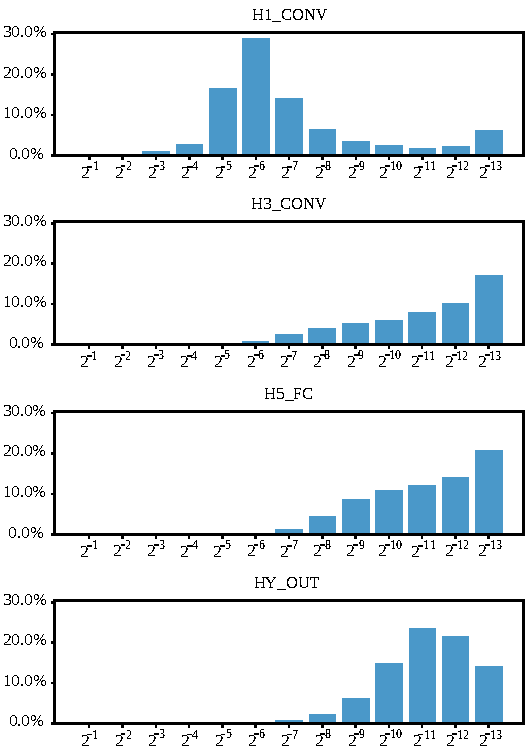
\includegraphics[width=\columnwidth]{../figures/log2_histogram.pdf}
	\caption{$\log_2$-histogram of each synaptic weight matrix showing the percentage of matrix elements with given integer exponent.}\label{fig:log2histogram}
\end{figure}

\subsubsection{Design exploration for dot-product using custom floating-point approximation}
For this design exploration, we use a custom floating-point representation composed of 4-bit exponent and 1-bit mantissa. This format is used for the synaptic weight vector on the proposed dot-product architecture. Each \emph{Conv} PU instantiates an on-chip stationary weight matrix for $52,000$ entries of 5-bit. The available memory size is large enough to store $W\in\mathbb{R}^{5\times 5\times 2\times 32}$ and $W\in\mathbb{R}^{5\times 5\times 32\times 64}$ for \emph{H1\_CONV} and \emph{H3\_CONV}, respectively. The same dot-product architecture is implemented in the processing unit of the fully connected layer (\emph{FC}). However, due to lack of block RAM (BRAM) resources, this PU can not instantiate on-chip stationary synaptic weight matrix. Instead, \emph{FC} receives the $\vec{W(s_t)}$ (weight vectors) during operation as well as $\vec{h_\mu}$ and $\vec{S_t}$. The hardware mapping and the computation schedule of this implementation are displayed in \Tab{tab:latency_cfp} and \Fig{fig:latency_pu_cfp_cycle}.

As shown in the computation schedule in \Tab{tab:latency_cfp} and \Fig{fig:latency_pu_cfp_cycle}, this implementation achieves a maximum hardware PU latency of $1.309 ms$ according to \equ{eq:time_pu}, and a CPU latency of $1.673 ms$. Therefore, applying \equ{eq:time_spike}, we obtain a latency of $1.673 ms$ per spike cycle as shown in \Fig{fig:latency_pu_cfp_cycle}. In this case, the cyclic bottleneck is in the performance of the CPU.

This configuration achieves an accuracy of $98.97\%$ correct classification on the $10,000$ image test set with $1000$ spikes. This indicates an accuracy degradation of $0.33\%$. For output quality monitoring, the noise tolerance plot in \fig{fig:accuracy_vs_noise_pu_cfp} revels accuracy degradation for noise higher than $50\%$ of amplitude, and convergence of inference after $400$ spikes. Thus, the particular SbS network implementation under approximate processing effects demonstrates a minimal impact on the overall accuracy. This proves an inherent error resilience, and hence, remaining approximation budget.

The post-implementation resource utilization and power dissipation are shown in \Tab{tab:resource_cfp} and \Tab{tab:power_cfp}, respectively.

\begin{table}[t!]\centering
	\caption{Performance of hardware processing units using custom floating-point approximation.}\label{tab:latency_cfp}
	\scriptsize
	\begin{tabular}{llrrrrrr}\toprule
		\multicolumn{2}{c}{\textbf{Hardware mapping}} & &\multicolumn{4}{c}{\textbf{Computation schedule (ms)}} \\\cmidrule{1-2}\cmidrule{4-7}
		\textbf{Layer} &\textbf{PU} & &$t_s$ &$t_{CPU}$ &$t_{PU}$ &$t_f$ \\\midrule
		HX\_IN &Spike & &0 &0.055 &0.307 &0.362 \\
		H1\_CONV &Conv1 & &0.057 &0.654 &1.309 &2.020 \\
		\multirow{2}{*}{H2\_POOL} &Pool1 & &0.713 &0.131 &1.098 &1.942 \\
		&Pool2 & &0.845 &0.125 &1.098 &2.068 \\
		\multirow{2}{*}{H3\_CONV} &Conv2 & &0.972 &0.285 &1.199 &2.456 \\
		&Conv3 & &1.258 &0.279 &1.184 &2.721 \\
		H4\_POOL &Pool3 & &1.538 &0.037 &0.484 &2.059 \\
		H5\_FC &FC & &1.577 &0.091 &0.438 &2.106 \\
		HY\_OUT &CPU & &1.669 &0.004 &0 &1.673 \\
		\bottomrule
	\end{tabular}
\end{table}

\begin{figure}[t!]
	\centering
	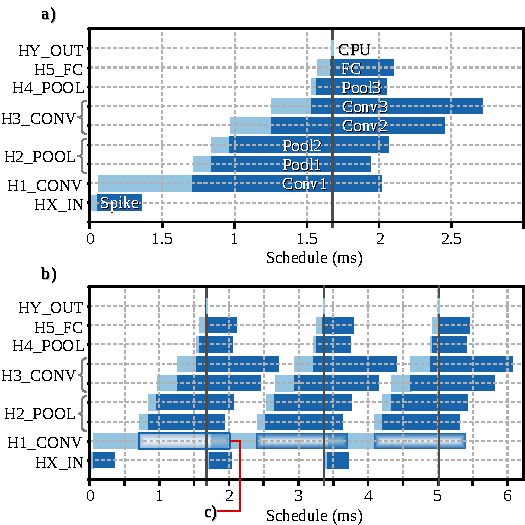
\includegraphics[width=1\columnwidth]{../figures/latency_cfp_cycle.pdf}
	\caption{Performance on processing units using custom floating-point approximation. a) Illustrates computation schedule. b) Illustrates cyclic computation schedule. c) Illustrates the performance of \emph{Conv2} from a previous computation cycle during the preprocessing of \emph{H1\_CONV} on the current computation cycle without bottleneck.}
	\label{fig:latency_pu_cfp_cycle}
\end{figure}

\begin{table}[h!]\centering
	\caption{Resource utilization of processing units using custom floating-point approximation.}\label{tab:resource_cfp}
	\scriptsize
	\begin{tabular}{lrrrrrr}\toprule
		\textbf{PU} & &\textbf{LUT} &\textbf{FF} &\textbf{DSP} &\textbf{BRAM 18K} \\\midrule
		Conv & &3,139 &4,850 &19 &25 \\
		FC & &3,265 &5,188 &8 &9 \\
		\bottomrule
	\end{tabular}
\end{table}

\begin{table}[h!]\centering
	\caption{Power dissipation of processing units using custom floating-point approximation.}\label{tab:power_cfp}
	\scriptsize
	\begin{tabular}{lrr}\toprule
		\textbf{PU} &\textbf{Power (mW)} \\\midrule
		Conv &82 \\
		FC &66 \\
		\bottomrule
	\end{tabular}
\end{table}

\begin{figure}[h!]
	\centering
	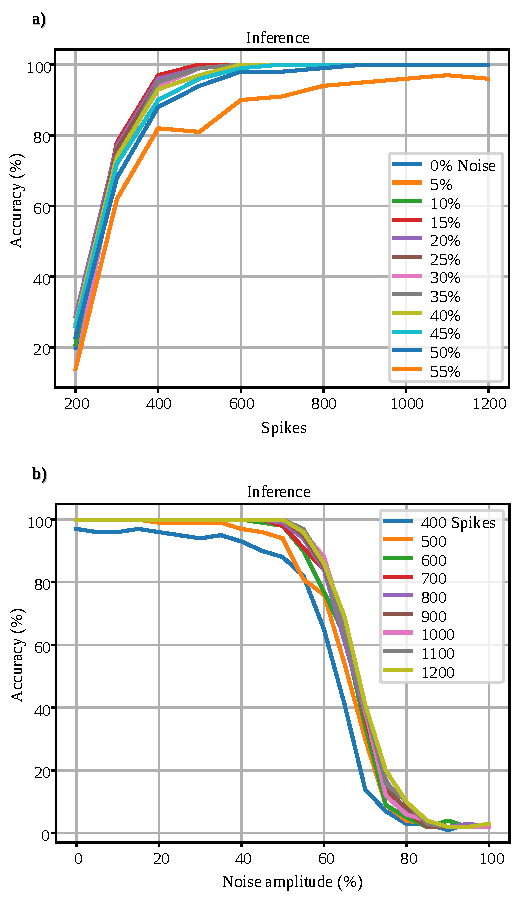
\includegraphics[width=1\columnwidth]{../figures/accuracy_vs_noise_pu_cfp(4-bit-exponent_1-bit-mantissa).pdf}
	\caption{Noise tolerance on hardware PU using custom floating-point approximation. (a) Illustrates accuracy degradation after $50\%$ of noise amplitude. (b) Illustrates convergence of inference after $400$ spikes.}
	\label{fig:accuracy_vs_noise_pu_cfp}
\end{figure}

\subsubsection{Design exploration for dot-product using logarithmic approximation}
As the worst-case quality configuration, we use a 4-bit integer exponent for logarithmic representation of the synaptic weight matrix. Each \emph{Conv} processing unit implements the proposed dot-product architecture including an on-chip stationary weight matrix for $52,000$ entries of 4-bit integer each one to store $W\in\mathbb{N}^{5\times 5\times 2\times 32}$ and $W\in\mathbb{N}^{5\times 5\times 32\times 64}$ for \emph{H1\_CONV} and \emph{H3\_CONV}, respectively. The same dot-product architecture is implemented in the \emph{FC} processing unit without stationary synaptic weight matrix. The hardware mapping and the computation schedule of this implementation are displayed in \Tab{tab:latency_log} and \Fig{fig:latency_pu_log_cycle}.

As shown in the computation schedule in \Tab{tab:latency_log} and \Fig{fig:latency_pu_log_cycle}, this implementation achieves a maximum hardware PU latency of $1.271 ms$ according to \equ{eq:time_pu}, and a CPU latency of $1.673 ms$. Therefore, applying \equ{eq:time_spike}, we obtain a latency of $1.673 ms$ per spike cycle as shown in \Fig{fig:latency_pu_log_cycle}. In this case, the cyclic bottleneck is in the CPU performance.

This quality configuration achieves an accuracy of $98.84\%$ correct classification on the $10,000$ image test set with $1000$ spikes. This indicates an accuracy degradation of $0.46\%$. For output quality monitoring, the noise tolerance plot in \fig{fig:accuracy_vs_noise_pu_log} revels accuracy degradation for noise higher than $40\%$ of amplitude, and convergence of inference after $600$ spikes. The particular SbS network implementation under approximate processing demonstrates a minor impact on the overall accuracy. This exhibits remaining budget for further approximate processing approaches.

The post-implementation resource utilization and power dissipation are shown in \Tab{tab:resource_cfp} and \Tab{tab:power_cfp}, respectively.

\begin{table}[t!]\centering
	\caption{Performance of hardware processing units using logarithmic approximation.}\label{tab:latency_log}
	\scriptsize
	\begin{tabular}{llrrrrrr}\toprule
		\multicolumn{2}{c}{\textbf{Hardware mapping}} & &\multicolumn{4}{c}{\textbf{Computation schedule (ms)}} \\\cmidrule{1-2}\cmidrule{4-7}
		\textbf{Layer} &\textbf{PU} & &$t_s$ &$t_{CPU}$ &$t_{PU}$ &$t_f$ \\\midrule
		HX\_IN &Spike & &0 &0.055 &0.264 &0.319 \\
		H1\_CONV &Conv1 & &0.057 &0.655 &1.271 &1.983 \\
		\multirow{2}{*}{H2\_POOL} &Pool1 & &0.714 &0.130 &1.074 &1.918 \\
		&Pool2 & &0.845 &0.126 &1.106 &2.077 \\
		\multirow{2}{*}{H3\_CONV} &Conv2 & &0.973 &0.285 &1.179 &2.437 \\
		&Conv3 & &1.258 &0.278 &1.176 &2.712 \\
		H4\_POOL &Pool3 & &1.538 &0.037 &0.488 &2.063 \\
		H5\_FC &FC & &1.577 &0.091 &0.388 &2.056 \\
		HY\_OUT &CPU & &1.669 &0.004 &0 &1.673 \\
		\bottomrule
	\end{tabular}
\end{table}

\begin{figure}[!t]
	\centering
	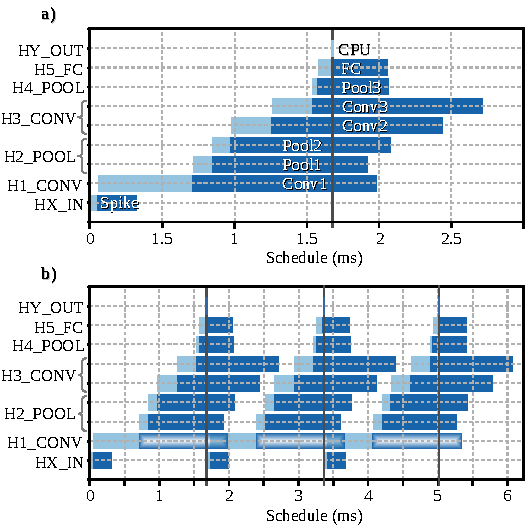
\includegraphics[width=1\columnwidth]{../figures/latency_log_cycle.pdf}
	\caption{Performance of processing units using logarithmic approximation. a) Illustrates computation schedule. b) Illustrates cyclic computation schedule.}
	\label{fig:latency_pu_log_cycle}
\end{figure}

\begin{table}[!h]\centering
	\caption{Resource utilization of processing units using logarithmic calculation.}\label{tab:resource_log}
	\scriptsize
	\begin{tabular}{lrrrrrr}\toprule
		\textbf{PU} & &\textbf{LUT} &\textbf{FF} &\textbf{DSP} &\textbf{BRAM 18K} \\\midrule
		Conv & &3,086 &4,804 &19 &21 \\
		FC & &3,046 &4,873 &8 &8 \\
		\bottomrule
	\end{tabular}
\end{table}

\begin{table}[!h]\centering
	\caption{Power dissipation of processing units using logarithmic calculation.}\label{tab:power_log}
	\scriptsize
	\begin{tabular}{lrr}\toprule
		\textbf{PU} &\textbf{Power (W)} \\\midrule
		Conv &78 \\
		FC &66 \\
		\bottomrule
	\end{tabular}
\end{table}

\begin{figure}[h!]
	\centering
	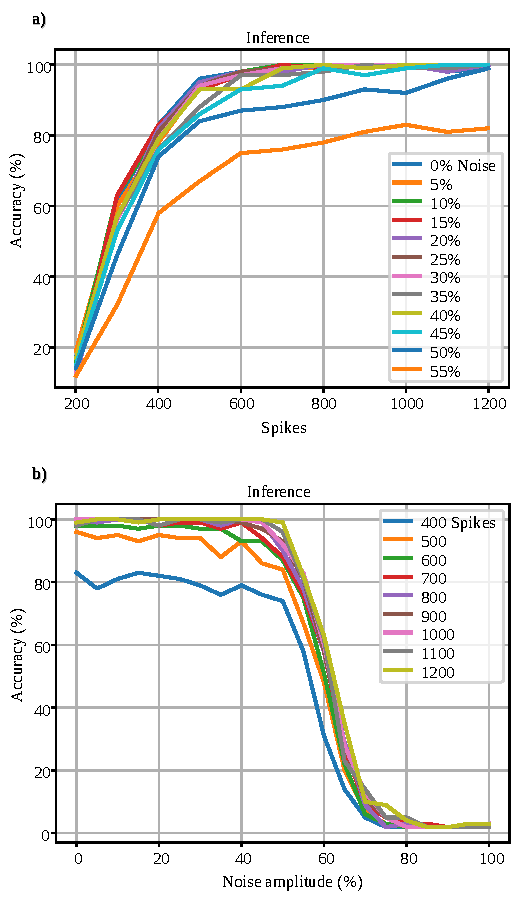
\includegraphics[width=1\columnwidth]{../figures/accuracy_vs_noise_pu_log.pdf}
	\caption{Noise tolerance on hardware PU using logarithmic approximation. (a) Illustrates accuracy degradation after $40\%$ of noise amplitude. (b) Illustrates convergence of inference after $600$ spikes.}
	\label{fig:accuracy_vs_noise_pu_log}
\end{figure}


\subsection{Results and discussion}
As a reference, the SbS network simulation on CPU using 32-bit standard floating-point achieves an accuracy of $99.3\%$ with a latency of $T_{SC} = 34.279ms$. As a second reference point, the network simulation on hardware processing units using standard floating-point achieves an accuracy of $98.98\%$ with a latency $T_{SC}=3.183ms$. As result we get a $10.77\times$ latency enhancement and an accuracy degradation of $0.32\%$. The tolerance plot in \fig{fig:accuracy_vs_noise_pu_fp} revels accuracy degradation when applying $50\%$ of input noise amplitude, and convergence of inference after $400$ spikes. In this case, the SbS network deployment with precise computing proves extraordinary inherent error resilience, and hence, vast approximation budget.

As a demonstration of the proposed dot-product architecture, the SbS network simulation on hardware PUs with synaptic representation using 5-bit custom floating-point (4-bit exponent, 1-bit mantissa) and 4-bit logarithmic (4-bit exponent) achieve $20.49\times$ latency enhancement and accuracy of $98.97\%$ and $98.84\%$, respectively. This results in an accuracy degradation of $0.33\%$ and $0.46\%$, respectively. For output quality monitoring, the noise tolerance plot in \fig{fig:accuracy_vs_noise_pu_cfp} and \fig{fig:accuracy_vs_noise_pu_log} revel accuracy degradation when applying $50\%$ and $40\%$ of input noise, and convergence of inference with $400$ and $600$ spikes, respectively. Therefore, the design exploration under the proposed approximate computing approach indicates sufficient inherent error resilience for further and more aggressive approximate processing approaches.

Regarding resource utilization and power dissipation, the \emph{Conv} processing units have a $43.24\%$ reduction of BRAM, and a $12.35\%$ of improvement in energy efficiency over the standard floating-point implementation. The experimental results of the design exploration are summarized in \Tab{tab:results}.

\begin{table*}[!t]
	\begin{threeparttable}
		\centering
		\caption{Experimental results of design exploration.}\label{tab:results}
		\scriptsize
		\begin{tabular}{lrrrrrrrrrrrrrrr}\toprule
			\multirow{2}{*}{\textbf{Implementation}} &\multirow{2}{*}{\textbf{PU}} &\multicolumn{4}{c}{\textbf{Post-implementation resource utilization}} & &\multirow{2}{*}{\textbf{Power (mW)}} & &\multicolumn{2}{c}{\textbf{Latency}} & &\multicolumn{3}{c}{\textbf{Accuracy (\%)\tnote{e}}} \\\cmidrule{3-6}\cmidrule{10-11}\cmidrule{13-15}
			& &\textbf{LUT} &\textbf{FF} &\textbf{DSP} &\textbf{BRAM 18K} & & & &$T_{SC}$ (ms) &\textbf{Gain\tnote{d}} & &\textbf{Noise 0\%} &\textbf{25\%} &\textbf{50\%} \\\midrule
			\multirow{2}{*}{Standard floating-point\tnote{a}} &Conv &2,765 &4,366 &19 &37 & &89 & &\multirow{2}{*}{3.183} &\multirow{2}{*}{10.77x} & &\multirow{2}{*}{98.98} &\multirow{2}{*}{98.96} &\multirow{2}{*}{98.63} \\
			&FC &2,649 &4,189 &8 &9 & &66 & & & & & & & \\
			& & & & & & & & & & & & & & \\
			\multirow{2}{*}{Custom floating-point\tnote{b}} &Conv &3,139 &4,850 &19 &25 & &82 & &\multirow{2}{*}{1.673} &\multirow{2}{*}{20.49x} & &\multirow{2}{*}{98.97} &\multirow{2}{*}{98.94} &\multirow{2}{*}{98.47} \\
			&FC &3,265 &5,188 &8 &9 & &66 & & & & & & & \\
			& & & & & & & & & & & & & & \\
			\multirow{2}{*}{Logarithmic\tnote{c}} &Conv &3,086 &4,804 &19 &21 & &78 & &\multirow{2}{*}{1.673} &\multirow{2}{*}{20.49x} & &\multirow{2}{*}{98.84} &\multirow{2}{*}{98.83} &\multirow{2}{*}{95.22} \\
			&FC &3,046 &4,873 &8 &8 & &66 & & & & & & & \\
			\bottomrule
		\end{tabular}
		\begin{tablenotes}
			\scriptsize
			\item[a] Synaptic storage composed of 4-bit exponent and 4-bit mantissa. For computation, each value is promoted to its standard floating-point representation.
			\item[b] Synaptic storage composed of 4-bit exponent and 1-bit mantissa.
			\item[c] Synaptic storage composed of 4-bit exponent.
			\item[d] Latency gain with respect to the CPU computation ($T_{SC} = 34.279 ms$).
			\item[e] Accuracy on 10,000 image test set at 1000 spikes.
		\end{tablenotes}
	\end{threeparttable}
\end{table*}